\section{Expansão de Taylor}

\begin{figure}[htb]
 \centering
 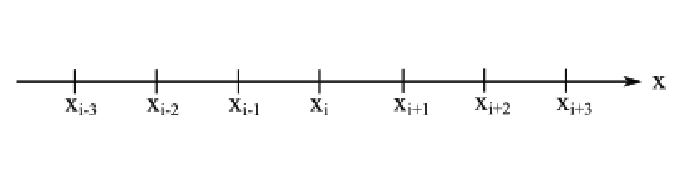
\includegraphics[scale=1.0]{capitulos/capitulo3/figuras/exp_taylor1.eps}
 \caption{?}
 \label{fig:exp_taylor1}
\end{figure}

\begin{equation}
 \label{cap3:sec1:eq1}
 f\,(x_{i+1}) = f\,(x_i+h) = f\,(x_i) + f'(x_i)\,h + \displaystyle \frac{1}{2}\,f''(x_i)\,h^2 + \frac{1}{6}\,f'''(x_i)\,h^3 + \frac{1}{24}\,f^{\,(iv)}\,h^4 \, \ldots
\end{equation}

\begin{equation}
 \label{cap3:sec1:eq2}
 f\,(x_{i-1}) = f\,(x_i-h) = f\,(x_i) - f'(x_i)\,h + \displaystyle \frac{1}{2}\,f''(x_i)\,h^2 - \frac{1}{6}\,f'''(x_i)\,h^3 + \frac{1}{24}\,f^{\,(iv)}\,h^4 + \ldots
\end{equation}

\begin{equation}
 \label{cap3:sec1:eq3}
 f\,(x_{i+2}) = f\,(x_i+2\,h) = f\,(x_i) + f'(x_i)\,2\,h + \displaystyle \frac{1}{2}\,f''(x_i)\,4\,h^2 + \frac{1}{6}\,f'''(x_i)\,8\,h^3 + \frac{1}{24}\,f^{\,(iv)}\,16\,h^4 + \ldots
\end{equation}

\begin{equation}
 \label{cap3:sec1:eq4}
 f\,(x_{i-2}) = f\,(x_i-2\,h) = f\,(x_i) - f'(x_i)\,2\,h + \displaystyle \frac{1}{2}\,f''(x_i)\,4\,h^2 - \frac{1}{6}\,f'''(x_i)\,8\,h^3 + \frac{1}{24}\,f^{\,(iv)}\,16\,h^4 + \ldots
\end{equation}

\begin{equation}
 \label{cap3:sec1:eq5}
 f\,(x_{i+3}) = f\,(x_i+3\,h) = f\,(x_i) + f'(x_i)\,3\,h + \displaystyle \frac{1}{2}\,f''(x_i)\,9\,h^2 + \frac{1}{6}\,f'''(x_i)\,27\,h^3 + \frac{1}{24}\,f^{\,(iv)}\,81\,h^4 + \ldots
\end{equation}

\begin{equation}
 \label{cap3:sec1:eq6}
 f\,(x_{i-3}) = f\,(x_i-3\,h) = f\,(x_i) - f'(x_i)\,3\,h + \displaystyle \frac{1}{2}\,f''(x_i)\,9\,h^2 + \frac{1}{4}\,f'''(x_i)\,27\,h^3 + \frac{1}{24}\,f^{\,(iv)}\,81\,h^4 + \ldots
\end{equation}

\begin{enumerar}
 \item Derivada Primeira (mínimo 2 pontos)

\begin{enumerar}
 \item \textit{Forward Difference}

2 pontos ($x_{i}$ e $x_{i+1}$)

De \ref{cap3:sec1:eq1}:

\[
 \begin{array}{l}
  f'(x_i) = \displaystyle \frac{f\,(x_{i+1}) - f\,(x_i)}{h} - \frac{1}{2} \, f''(x_i) \, h - \frac{1}{6}\,f'''(x_i)\,h^2 - \ldots \vspace*{0.2cm} \\
  f'(x_i) = \displaystyle \frac{f\,(x_{i+1}) - f\,(x_i)}{h} + O\,(h)
 \end{array}
\]

onde

\[
 O\,(h) = -\frac{1}{2}\,f''(x_i)\,h
\]

3 pontos ($x_{i}$, $x_{i+1}$ e $x_{i+2}$)

De -(\ref{cap3:sec1:eq3}) + 4*(\ref{cap3:sec1:eq1}):

\[
 4\,f\,(x_{i+1}) - f\,(x_{i+2}) = 3\,f\,(x_i) + 2\,h\,f'(x_i) - \frac{2}{3}\,h^3\,f'''(x_i)
\]

\[
 f'(x_i) = \frac{-f\,(x_{i+2}) + 4\,f\,(x_{i+1}) - 3\,f\,(x_i)}{2\,h} + O\,(h^2)
\]

onde

\[
 O\,(h^2) = \frac{1}{3} \, h^2 \, f'''(x_i)
\]

4 pontos ($x_{i}$, $x_{i+1}$, $x_{i+2}$ e $x_{i+3}$)

De (\ref{cap3:sec1:eq1}) - $\displaystyle \frac{1}{2}$*(\ref{cap3:sec1:eq3}) + $\displaystyle \frac{1}{9}$*(\ref{cap3:sec1:eq5}):

\[
 \begin{array}{c}
 \underline{
 \begin{array}{rcrrrrrr}
    f_{i+1} & = & f_i & + h\,f'_i & + \displaystyle \frac{h^2}{2} \, f''_i & + \displaystyle \frac{h^3}{6} \, f'''_i & + \displaystyle \frac{h^4}{24} \, f''''_i & + \ldots \vspace*{0.2cm} \\
  - \displaystyle \frac{f_{i+2}}{2} & = & - \displaystyle \frac{f_i}{2} & - h\,f'_i & - \displaystyle \frac{2\,h^2}{2}\,f''_i & - \displaystyle \frac{4\,h^3}{6} \, f'''_i & - \displaystyle \frac{8\,h^4}{24}\,f'''' & - \ldots \vspace*{0.2cm} \\
  + \displaystyle \frac{f_{i+3}}{9} & = & \displaystyle \frac{f_i}{9} & + \displaystyle \frac{h}{3}\,f'_i & + \displaystyle \frac{h^2}{2}\,f''_i & + \displaystyle \frac{3\,h^3}{6}\,f'''_i & + \displaystyle \frac{9\,h^4}{24}\,f'''' & + \ldots
 \end{array}
 } \\
 \displaystyle \frac{f_{i+3}}{9} - \displaystyle \frac{f_{i+2}}{2} + f_{i+1} = \displaystyle \frac{f_i}{9} - \displaystyle \frac{f_i}{2} + f_i + \displaystyle \frac{h}{3}\,f'_i + \displaystyle \frac{h^4}{12}\,f'''' + \ldots
 \end{array}
\]

\[
 f'_i = \frac{2\,f_{i+3} - 9\,f_{i+2} + 18\,f_{i+1} - 11\,f_i}{6\,h} + O\,(h^3)
\]

onde

\[
 O\,(h^3) = - \frac{1}{4} \, h^3 \, f''''_i
\]

\item \textit{Backward Difference}

2 pontos ($x_{i}$ e $x_{i-1}$)

De (\ref{cap3:sec1:eq2}):

\[
 f'(x_i) = \frac{f\,(x_i) - f\,(x_{i-1})}{h} + O\,(h)
\]

onde

\[
 O\,(h) = \frac{1}{2}\,f''(x_i)\,h
\]

3 pontos ($x_{i}$, $x_{i-1}$ e $x_{i-2}$)

\[
 f'(x_i) = \frac{3\,f\,(x_i) - 4\,f\,(x_{i-1}) + f\,(x_{i-2})}{2\,h} + O\,(h^2)
\]

onde

\[
 O\,(h^2) = \frac{1}{3}\,h^2\,f'''(x_i)
\]

4 pontos ($x_{i}$, $x_{i-1}$, $x_{i-2}$ e $x_{i-3}$)

\[
 f'(x_i) = \frac{11\,f_i - 18\,f_{i-1} + 9\,f_{i-2} - 2\,f_{i-3}}{6\,h} + O\,(h^3)
\]

onde

\[
 O\,(h^3) = \frac{1}{4}\,h^3\,f''''_i
\]

\item \textit{Central Difference}

2 pontos ($x_{i+1}$ e $x_{i-1}$)

De (\ref{cap3:sec1:eq1}) - (\ref{cap3:sec1:eq2}):

\[
 f'(x_i) = \frac{f\,(x_{i+1}) - f\,(x_{i-1})}{2\,h} + O\,(h^2)
\]

onde

\[
 O\,(h^2) = -\frac{1}{6}\,h^2\,f'''(x_i)
\]

4 pontos ($x_{i+2}$, $x_{i+1}$, $x_{i-1}$ e $x_{i-2}$) (elimine $f''$ $f'''$)

\[
 f'_i = \frac{-f_{i+2} + 8\,f_{i+1} - 8\,f_{i-1} + f_{i-2}}{12\,h} + O\,(h^2)
\]

onde

\[
 O\,(h^2) = \frac{1}{30} \, h^4 \, f^{\,(iv)}(x_i)
\]

 \end{enumerar}

\item Derivada Segunda (mínimo 3 pontos)

\begin{enumerar}

\item \textit{Forward Difference}

3 pontos ($x_{i}$, $x_{i+1}$ e $x_{i+2}$) elimina $f'(x_{i})$

\[
 f''_i = \frac{f_{i+2} - 2\,f_{i+1} + f_i}{h^2} + O\,(h)
\]

onde

\[
 O\,(h) = -h\,f'''_i
\]

\item \textit{Backward Difference}

\[
 f''_i = \frac{f_i - 2\,f_{i+1} + f_{i-2}}{h^2} + O\,(h)
\]

onde

\[
 O\,(h) = h\,f'''_i
\]

\item \textit{Central Difference}

\[
 f''_i = \frac{f_{i+1} - 2\,f_i + f_{i-1}}{h^2} + O\,(h^2)
\]

onde

\[
 O\,(h^2) = -\frac{1}{2}\,h^2\,f''''_i
\]

\end{enumerar}

\end{enumerar}

\textbf{OBS:}

\begin{itemize}
 \item Uma aproximação para $f^{(p)}$ precisa de pelo menos $p+1$ pontos.

\item As derivadas de ordem menor do que $p$ devem ser eliminadas.

\item O erro é o termo de ordem mais baixa que for truncado.

\end{itemize}

